\documentclass[11pt,a4paper]{article} 

\usepackage{titlesec}
\usepackage{color}
\usepackage[utf8]{inputenc}
\usepackage[english]{babel}
\usepackage[T1]{fontenc}
\usepackage{graphicx}
\graphicspath{{Images/}}
\usepackage{eso-pic} 
\usepackage{subfig} 
\usepackage{caption}
\usepackage{transparent}

% STANDARD MATH PACKAGES
\usepackage{amsmath}
\usepackage{amsthm}
\usepackage{bm}
\usepackage[overload]{empheq} 

% PACKAGES FOR TABLES
\usepackage{tabularx}
\usepackage{colortbl}

% PACKAGES FOR ALGORITHMS (PSEUDO-CODE)
\usepackage{algorithm}
\usepackage{algorithmic}

% PACKAGES FOR REFERENCES & BIBLIOGRAPHY
\usepackage[colorlinks=true,linkcolor=black,anchorcolor=black,citecolor=black,filecolor=black,menucolor=black,runcolor=black,urlcolor=black]{hyperref} % Adds clickable links at references
\usepackage{cleveref}
\usepackage[square, numbers, sort&compress]{natbib} 

\bibliographystyle{plain} % You may use a different style adapted to your field

% PACKAGES FOR THE APPENDIX
\usepackage{appendix}

% PACKAGES FOR ITEMIZE & ENUMERATES 
\usepackage{enumitem}

% OTHER PACKAGES
\usepackage{amsthm,thmtools,xcolor} % Coloured "Theorem"
\usepackage{fancyhdr} % Fancy headers and footers
\usepackage{lipsum} % Insert dummy text
\usepackage{tcolorbox} % Create coloured boxes


% Do not change Configuration_files/config.tex file unless you really know what you are doing.
%DO NOT EDIT
% Configuration package
\usepackage[bottom=2.0cm,top=2.0cm,left=2.0cm,right=2.0cm]{geometry}
\raggedbottom 

\definecolor{newblue}{cmyk}{0.4,0.1,0,0.4}

% Custom theorem environments
\declaretheoremstyle[
  headfont=\color{newblue}\normalfont\bfseries,
  bodyfont=\color{black}\normalfont\itshape,
]{colored}

\captionsetup[figure]{labelfont={color=newblue}} 
\captionsetup[table]{labelfont={color=newblue}} 
\captionsetup[algorithm]{labelfont={color=newblue}} 

\theoremstyle{colored}
\newtheorem{theorem}{Theorem}[section]
\newtheorem{proposition}{Proposition}[section]

\newcommand\T{\rule{0pt}{2.6ex}}
\newcommand\B{\rule[-1.2ex]{0pt}{0pt}}

\newcounter{algsubstate}
\renewcommand{\thealgsubstate}{\alph{algsubstate}}
\newenvironment{algsubstates}{
    \setcounter{algsubstate}{0}%
    \renewcommand{\STATE}{%
    \stepcounter{algsubstate}%
    \Statex {\small\thealgsubstate:}\space}
    }{}
    
% Custom theorem environment
\newcolumntype{L}[1]{>{\raggedright\let\newline\\\arraybackslash\hspace{0pt}}m{#1}}
\newcolumntype{C}[1]{>{\centering\let\newline\\\arraybackslash\hspace{0pt}}m{#1}}
\newcolumntype{R}[1]{>{\raggedleft\let\newline\\\arraybackslash\hspace{0pt}}m{#1}}

% Custom itemize environment
\setlist[itemize,1]{label=$\bullet$}
\setlist[itemize,2]{label=$\circ$}
\setlist[itemize,3]{label=$-$}
\setlist{nosep}


\setlength\parindent{0pt}

% Custom title commands
\titleformat{\section}
{\color{newblue}\normalfont\Large\bfseries}
{\color{newblue}\thesection.}{1em}{}
\titlespacing*{\section}
{0pt}{3.3ex}{3.3ex}

\titleformat{\subsection}
{\color{newblue}\normalfont\large\bfseries}
{\color{newblue}\thesubsection.}{1em}{}
\titlespacing*{\subsection}
{0pt}{3.3ex}{3.3ex}

% Custom headers and footers
\pagestyle{fancy}
\fancyhf{}
      
\fancyfoot{}
\fancyfoot[C]{\thepage} % page
\renewcommand{\headrulewidth}{0mm} % headrule width
\renewcommand{\footrulewidth}{0mm} % footrule width

\makeatletter
\patchcmd{\headrule}{\hrule}{\color{black}\hrule}{}{} % headrule
\patchcmd{\footrule}{\hrule}{\color{black}\hrule}{}{} % footrule
\makeatother

% Insert here the info that will be displayed into your Title page 
\renewcommand{\title}{Suffix Trees}
\newcommand{\authorA}{Aditya Patil (2021CSB1062)}
\newcommand{\authorB}{Alankrit Kadian (2021CSB1065)}
\newcommand{\authorC}{Harsh Raj Srivastava (2021CSB1091)} %comment if not needed
%\newcommand{\authorD}{Student4Name (ID4)} %comment if not needed
\newcommand{\advisor}{Dr. Anil Shukla}
\newcommand{\firstcoadvisor}{Akanksha}
\newcommand{\summary}{We have first performed and analysed the construction of the suffix tree in linear time using the \emph{Ukkonen's algorithm}. We also implemented our own thought application of suffix trees in which we also incorporated \emph{BK-Tree} and \emph{Bloom Filter}. We designed a simple system to keep track of grocery item orders and generate a order reciept and also handle queries of each item for the seller(using the linear search operation of suffix trees). We call this a simple grocery shop management system.}

%-------------------------------------------------------------------------
%	BEGIN OF YOUR DOCUMENT
%-------------------------------------------------------------------------
\begin{document}

% Do not change Configuration_files/TitlePage.tex
% DO NOT EDIT


\null\hfill
\includegraphics[width=0.2\textwidth]{Images/IIT_Rpr_logo.jpg}

\vspace{3mm}
\Large{\textbf{\color{newblue}{\title}}}
\vspace{0.1cm}\\
\null\hfill \today\\
\large{\textbf{\authorA}}\vspace{1mm}
,\\ \large{\textbf{\authorB}}\vspace{1mm}
\ifdefined \authorC
,\\ \large{\textbf{\authorC}}\vspace{1mm}
\ifdefined \authorD
,\\ \large{\textbf{\authorD}}\vspace{1mm}
\fi 
\fi
\small \normalfont

\vspace{11pt}

\centerline{\rule{1.0\textwidth}{0.4pt}}

\begin{center}
\begin{minipage}[t]{.24\textwidth}
\begin{minipage}{.90\textwidth}
\noindent
\footnotesize{\textbf{Instructor:} \\
\advisor} \\
\\
\footnotesize{\textbf{Teaching Assistant:}\\ 
\firstcoadvisor}\\ 

\end{minipage}
\end{minipage}
\begin{minipage}{.74\textwidth}
\noindent \textbf{\color{newblue} Summary:} {\summary}
\end{minipage}
\end{center}

\vspace{8pt}

\centerline{\rule{1.0\textwidth}{0.4pt}}
\vspace{12pt}
%Main Text starting point
\section{Suffix Trees}
\label{sec:introduction}
A suffix tree is a data structure that exposes the internal structure of a string. Suffix trees are useful in various string processing and computational problems. They provide linear-time solutions to many complex string problems, after just O(m), or linear, preprocessing time for a given string of length m. Applications of suffix trees include exact matching problem, substring problem, pattern searching, longest repeating substring, building linear time suffix array, longest common substring, longest palindromic substring, etc.
\\
\\
\textbf{Definition:} A suffix tree \begin{math}\tau\end{math} for an m-character string S is a rooted directed tree with exactly m leaves indexed 1 to m. For any leaf i, the concatenation of the edge-labels on the path from the root to leaf i exactly spells out the suffix of S that starts at position i, i.e. S[i...m]. Each internal node, other than the root, has at least two children and each edge is labeled with a non-empty substring of S. No two edges out of the same node can have edge-labels beginning with the same character.
The \emph{label of a path} from the root that ends at a node is the concatenation in order, of the substrings labeling the edges of that path. The \emph{path label} of a node is the label of the path from the root to that node.
\\
\\
For example, let us take a look at the suffix tree for string S = "xabxac" which have six suffixes, namely "xabxac", "abxac", "bxac", "xac, "ac" and "c".
\begin{figure}[H]
    \centering
    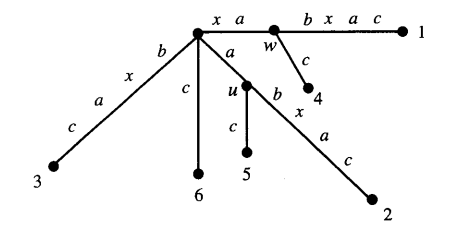
\includegraphics{Images/image1.png}
    \caption{Suffix Tree for string S = "xabxac"}
    \label{fig:suffixtreeExample}
\end{figure}
As shown in Figure 1, the suffix tree for string S has one root node, two internal nodes and six leaf edges representing each of its six suffixes.
\\
The above definition of a suffix tree for S does not gaurantee that the suffix tree for any string S actually exists. The problem is that if one suffix of S matches the prefix of another suffix of S, then no suffix tree obeying the above definition is possible. To avoid this problem, we have to assume that the last character of S appears nowhere else in S, so that no suffix of the resulting string can be a prefix of any other suffix. To achieve this in practice, we can add a character, like `\$', to the end of S that is not present in S already. This is called the \emph{termination character}. 

\subsection{Construction Of Suffix Tree}
There are various algorithms to build a suffix tree for a string S. First, we will present a straightforward algorithm which takes \begin{math}O(m^2)\end{math} time to build the suffix tree for a string S of length m, and then we will see another algorithm which, with some observations, tricks and implementation speedups, will build the suffix tree for us in linear i.e. \begin{math}O(m)\end{math} time.

\subsubsection{A naive algorithm to build a suffix tree}
\label{subsec:naivealgorithm}
This naive method first enters a single edge for suffix S[1...m]\$(the entire string) into the tree, and then it successively enters suffix S[i...m]\$ into the growing tree, for 2 $\le$ i $\le$ m. Let \begin{math}\tau\end{math}\textsubscript{i} denote the intermediate tree that encodes all the suffixes from 1 to i. 
\\
Tree \begin{math}\tau\end{math}\textsubscript{1} consists of a single edge between the root of the tree and a leaf labeled 1 and the edge is labeled with the string S\$. Tree \begin{math}\tau\end{math}\textsubscript{i+1} is constructed from \begin{math}\tau\end{math}\textsubscript{i} as follows:
\\
Starting at the root of \begin{math}\tau\end{math}\textsubscript{i}, find the longest path by successively comparing and matching characters from the root whose label matches a prefix of S[i+1...m]\$. The matching path will be unique as no two edges out of a node can have labels that begin with the same character. The matching path either ends at a node, say w, or it ends in the middle of an edge. If it is in the middle of an edge, say (u,v), then it breaks the edge (u,v) into edges by inserting in a new node, say w, just after the last character on that edge that mismatched. The new edge (u,w) is labeled with the part of (u,v) label that matched with S[i+1...m], and the new edge (w,v) is labeled with the remaining part of the (u,v) label. A new edge (w,i+1) running from w to a new leaf labeled i+1 is created, and it is labeled with the unmatched part of suffix S[i+1...m]\$. The suffix tree now contains a unique path from root to leaf i+1 with path label S[i+1...m]\$.
\\
As mentioned earlier, the naive method takes \begin{math}O(m^2)\end{math}
time to build a suffix tree for the string S of length m.

\subsubsection{Ukkonen's linear-time suffix tree algorithm}
\label{subsec:ukknalgorithm}
Esko Ukkonen devised a linear-time algorithm for constructing a suffix tree that, with its "on-line" property and the simplicity of its description, proof, and time analysis, may be the conceptually easiest linear-time construction algorithm. 
\paragraph{Implicit suffix trees}
While constructing suffix trees using Ukkonen's algorithm, we will see `implicit suffix tree' in some intermediate steps depending on characters in string S.
\\
An \emph{implicit suffix tree} for string S is a tree obtained from the suffix tree for S\$ by removing every copy of the termination character \$ from the edge labels of the tree, then removing any edge that has no label, and then removing any node that does not have two or more children. Even though an implicit suffix tree may not have a leaf for each suffix, it does encode all the suffixes of S, as each suffix is spelled out by the characters on some path from the root of the implicit suffix tree. But implicit suffix trees are less informative than true suffix trees than true suffix trees as there's no marker for suffixes of S whose path does not end at a leaf. So, we will just use them as a tool in Ukkonen's algorithm to finally obtain the true suffix tree for string S.
\paragraph{Ukkonen's algorithm at a high level}
Ukkonen's algorithm is divided into m \emph{phases}, where m is the length of the string. In phase i+1, tree \begin{math}\tau\end{math}\textsubscript{i+1} is constructed from \begin{math}\tau\end{math}\textsubscript{i}, and each phase i+1 is divided into i+1 \emph{extensions}, one for each of the i+1 suffixes of \begin{math}S[1...i+1]\end{math}. In extension j of phase i+1, the algorithm finds the end of the path from the root labeled with \begin{math}S[j...i]\end{math} and extends the substring by adding \begin{math}S[i+1]\end{math} to the end (unless \begin{math}S[i+1]\end{math} is already there).
\begin{algorithm}[H]
\caption*{High-Level Ukkonen's Algorithm}
\label{ukknathighlevelpsuedocode}
\begin{algorithmic}
\STATE Construct tree \begin{math}\tau\end{math}\textsubscript{1},
\FOR{$1 \leq i \leq m-1$}
\STATE begin {phase i+1}
\FOR{$1 \leq j \leq i+1$}
\STATE begin {extension j}
\STATE find the end of the path from the root labeled \begin{math}S[j...i]\end{math} in the current tree. Extend the path by adding \begin{math}S[i+1]\end{math} (if not already there) thus putting the string \begin{math}S[j...i+1]\end{math} into the suffix tree.
\ENDFOR
\ENDFOR
\end{algorithmic}
\end{algorithm}
\textbf{Suffix Extension Rules}
\\
In extension j, the algorithm finds the end of suffix \begin{math}S[j...i]\end{math} in the current tree, and extends \begin{math}S[j...i]\end{math} to be sure the suffix \begin{math}S[j...i+1]\end{math} is in the tree. This is done according to one of the following three rules:
\\
\emph{Rule 1}: If the path for \begin{math}S[j...i]\end{math} extends to the end of a leaf edge, then \begin{math}S[i+1]\end{math} is simply added to the end of the label of that leaf edge.
\\
\emph{Rule 2}: If no path from the end of \begin{math}S[j...i]\end{math} starts with \begin{math}S[i+1]\end{math}, but atleast one labeled path continues from the end of \begin{math}S[j...i]\end{math}, then a new leaf edge starting from the end of \begin{math}S[j...i]\end{math} is created and labeled \begin{math}S[i+1]\end{math}. A new internal node is also created if the path for \begin{math}S[j...i]\end{math} ends in the middle of an edge.
\\
\emph{Rule 3}: If a path from the end of \begin{math}S[j...i]\end{math} starts with \begin{math}S[i+1]\end{math}, then the string \begin{math}S[j...i+1]\end{math} is already in the suffix tree, and thus we do nothing.

\paragraph{Implementation Speedups}
The above method takes \begin{math}O(m^3)\end{math} to build the suffix tree and the Ukkonen's algorithm is a speedup of this method. The key issue in implementing Ukkonen's algorithm is to how to locate the ends of all the $i+1$ suffixes of $S[1...i]$.
\\
\\
\textbf{Suffix links}
\\
Let $x\alpha$ denote an arbitrary string, where $x$ denotes a single character and $\alpha$ denotes a substring of S (possibly empty). For an internal node $v$ with path label $x\alpha$, if there is another node $s(v)$ with path label $\alpha$, then a pointer from $v$ to $s(v)$ is called a \emph{suffix link}.
\\
Suffix links provide a short cut to find end of the path S[j...i]. We can start from the end of path S[j-1...i], walk up one edge to node v, follow the suffix link to s(v), then walk down the path. 
\\
\\
\textbf{Skip/Count trick}
\\
When walking down from node \begin{math}s(v)\end{math} to leaf, instead of matching path character by character as we travel, we can directly skip to the next node if number of characters on the edge is less than the number of characters we need to travel.
\\
\\
\textbf{Edge-label compression}
\\
So far, path labels are represented as characters in string, but a simple, alternate scheme exists for edge labeling. Instead of explicitly writing a substring on an edge of the tree, only write a pair of indices on the edge, specifying beginning and end positions of that substring in S (see Figure 3).
\\
\\
\textbf{Extension rule 3 as a show stopper}
\\
In any phase, if suffix extension rule 3 applies in extension j, it will also apply in all further extensions i.e. extension j to i+1, until the end of the phase. So, we will end any phase the first time that extension rule 3 applies. All the extensions from there on are said to be done \emph{implicitly}. All previous extensions of that phase are said to be done \emph{explicitly}.
\\
\\
\textbf{A leaf always remains a leaf}
\\
If at some point in Ukkonen's algorithm a leaf is created and labeled j (for the suffix starting at position j of S), then that leaf will remain a leaf in all successive trees created during the algorithm. Once there is a leaf labeled j, extension rule 1 will always apply to extension j all successive phases. So, in phase i+1, when a leaf edge is first created and would be labeled with substring S[p...i+1], instead of writing indices (p,i+1) on that edge, write (p,e), where e is the 'current end' which is a global index set to i+1 once in each phase i+1.
\\
\\
\textbf{Active point}
\\
Any phase i goes through a series of j extensions ($1 \leq j \leq i$), in which first p ($0 \leq p < i$) extensions will follow Rule 1, next q ($0 \leq q \leq i-p$) extensions will follow Rule 2 and next r ($0 \leq r \leq 1$) extensions will follow Rule 3. The order in which Rule 1, Rule 2 and Rule 3 apply, is never intermixed in any phase. At the end of any phase i, there will be $j_i$ = p+q leaf edges and next phase i+1 will go through Rule 1 for first $j_i$ extensions. It follows from previous observation (a leaf always remains a leaf) that for each $1 \leq i \leq m-1$, $j_i \leq j_i+1$.
\\
For further extensions, we need to explicitly add the new character at the end of the best possible matching edge. This is where active point comes into play, which is the point where the same extension of the last phase ended. Active point helps to avoid unnecessary path traversals from root in any extension based on the knowledge gained in traversals in the previous extension. For the 1st extension of phase 1, active point is set to the root, and other extensions will get active point set correctly by previous extension. Active point is updated at the end of each extension according to some rules like, active point change for extension rule 3(APCFER3), for extension rule 2(APCFER2C1 \& APCFER2C2), for walk down(APCFWD) and for active point at a node(APCFALZ).
\\
\\
Using all the implementation tricks, \emph{Ukkonen's algorithm} builds the implicit suffix trees \begin{math}\tau\end{math}\textsubscript{1} through \begin{math}\tau\end{math}\textsubscript{m} in \begin{math}O(m)\end{math} total time. We look at the algorithm through two sub-algorithms shown below.
\begin{algorithm}[H]
\caption*{Single extension algorithm}
\label{seapsuedocode}
\begin{algorithmic}
\STATE Begin {extension $j$} 
\STATE 1. We have to find the first node v at or above the end of $S[j-1...i]$ that either has a suffix link from it or is the root. Active node is exactly that node. Let $\gamma$ (possibly empty) denote the string between v and the end of $S[j-1...i]$.
\STATE 2. If $v$ is not the root, traverse the suffix link from v to node s(v) and then walk down from $s(v)$ following the path for string $\gamma$. If v is the root, then follow the path for $S[j...i]$ from the root.
\STATE 3. Using the extension rules, ensure that the string $S[j...i]S[i+1]$ is in the tree.
\STATE 4. If a new internal node $w$ was created in extension $j-1$ (by extension rule 2), create the suffix link $(w,s(w))$ from $w$ to $s(w)$.
\STATE 5. Update the active point for the next extension.
\STATE End
\end{algorithmic}
\end{algorithm}

\begin{algorithm}[H]
\caption*{Single phase algorithm}
\label{spapsuedocode}
\begin{algorithmic}
\STATE Begin {phase $i+1$}
\STATE 1. Increment index e to $i+1$(For directly applying Rule 1 for extensions 1 through $j_1$).
\STATE 2. Explicitly compute successive extensions (using single extension algorithm) starting at $j_i+1$ until reaching the first extension, say $j^*$, where rule 3 applies or until extensions are done in this phase. (this correctly implements all the additional implicit extensions $j^*+1$ through $i+1$).
\STATE 3. Set $j_{i+1}$ to $j^*-1$, to prepare for the next phase.
\STATE End
\end{algorithmic}
\end{algorithm}

The final implicit suffix tree $\tau_m$ can be converted to a true suffix tree in $O(m)$ time by adding the termination character '\$' to the end of S and let Ukkonen's algorithm continue with this character. The other change needed is to replace each index e on every leaf edge with the number m and also assign suffix index to each leaf. This is achieved by an $O(m)$ time traversal of the tree, visiting each leaf edge. The resulting suffix tree is a true suffix tree.

\section{Bloom Filter}
\label{sec:bloomfilter}
A \emph{bloom filter} is a space-efficient probabilistic data structure which is used to maintain a set of strings we certainly know are unique. 
For this, we use a number of \emph{hash functions} and a boolean array.
A small flaw associated with the use of the bloom filter is that there can be false positives i.e. sometimes a element would not have been previously entered but the bloom filter would tell otherwise. This can be minimized by choosing a large boolean array and a good choice of hash functions. Let's say there are k hash functions $h_1, h_2, h_3,..., h_k$, and string s.
These hash functions take a string as an argument and map it to an integer.
Then we create a large boolean array of size say m, and set the bits $h_1(s), h_2(s), h_3(s),..., h_k(s)$ in the boolean array.
We can do two operations with the bloom filter, namely: 
\\
\textbf{Insert}: To insert an element in the bloom filter by setting the bits corresponding to the element.
\\
\textbf{Lookup}: To check whether an element is already present in bloom filter with a positive false probability.
\\
The fundamental idea of bloom filter is that if all the bits are set it means that there is a good chance that the word was already inserted and it will output that the element is probably present, else surely the element was not inserted.
\\
Bloom filter can sometimes give false positives but can never give false negatives.
Unlike a standard hash table, a bloom filter of a fixed size can represent a set with an arbitrarily large number of elements.

\section{BK Tree}
\label{sec:bktree}
\emph{BK Trees}, or Burkhard-Keller Trees are a tree-based data structure made for quickly finding near-matches to a string, for example, as a spell checker. It is based on the concept of \emph{Levenshtein distance}, or simply `edit-distance' which is the number of edits (operations: insert, remove, replace) required to convert one string to another.
\\
First, we have a dictionary of strings on which we build the BK Tree. The structure of BK Tree is like any other tree i.e. it consists of nodes and edges. The nodes represent individual words and the edge contains some integer weight that is the edit distance from one node to another. Every node in the BK Tree will have exactly one child with same edit-distance. An example of BK Tree is shown in figure below.
\begin{figure}[H]
    \centering
    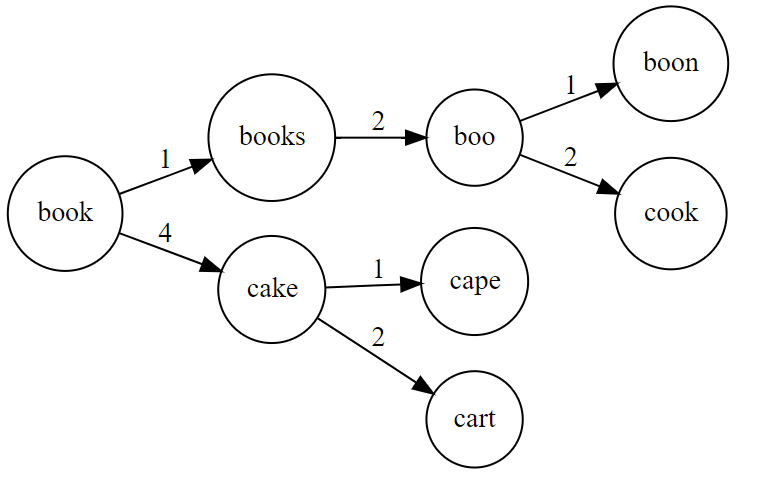
\includegraphics{Images/image2.png}
    \caption{BK Tree example}
    \label{fig:bktreeExample}
\end{figure}
Now, to find the closest correct word for a given word, we have to set a tolerance value which is simply the maximum edit distance from our word to the correct words in our dictionary.
\\
The time complexity will be $O(L_1*L_2*log(n))$ where $L_1$ is the average length of the word in our dictionary, $L_2$ is the length of the given word and n is the size of the dictionary.

\section*{Application}
\paragraph{Aim}
To design a simple \emph{Grocery Shop Management System}.
\\
\textbf{What exactly will it do?}
\\
This can be divided into three parts.
\\
\textbf{Part 1:} In first part of the system, we take grocery items as input from the seller and our program keeps track of those items. The set of items maintained will each be unique, and we keep sure of that using the bloom filter.
\\
\textbf{Part 2:} In second part of the system, different consumers input items that they want. In case, the consumer makes a spelling mistake, there the BK Tree comes in to find the closest matching item (if there is one). 
\\
\textbf{Part 3:} In third part of the system, an order reciept of all items ordered by different consumers is generated for seller's reference. In this we use suffix trees to find all the occurences of each item ordered by the consumers.

\section{Conclusions}
\color{black}
In this project, we see that suffix tree is the best data structure particularly for fast implementations of many important string operations. We also implement two other data structures, bloom filter and BK-tree, that help us in preventing repetitions in the grocery items list and auto-correcting the order items entered by consumers, respectively. So, using three data structures, we implement an efficient grocery shop management system that searches orders for specific items in linear time i.e. of the order of the string length of the item.

\section{References}
\label{sec:refrnces}
1) https://www.cs.cmu.edu/afs/cs/project/pscico-guyb/realworld/www/slidesF06/cmuonly/gusfield.pdf
\\
2) https://en.wikipedia.org/wiki/Suffix\_tree
\\
3) https://en.wikipedia.org/wiki/Ukkonen
\\
4) https://www.geeksforgeeks.org, Ukkonen's Suffix Tree Construction, Part 1-6
\\
5) https://www.geeksforgeeks.org/pattern-searching-using-suffix-tree/
\\
6) https://www.geeksforgeeks.org/bloom-filters-introduction-and-python-implementation/
\\
7) https://www.geeksforgeeks.org/bk-tree-introduction-implementation/
\\
8) http://blog.notdot.net/2007/4/Damn-Cool-Algorithms-Part-1-BK-Trees
\\
\end{document}